\documentclass{article}
\usepackage[final,main]{neurips_2025}

% Required packages
\usepackage[hidelinks]{hyperref}
\usepackage{booktabs}
\usepackage{graphicx}
\usepackage{amsmath,amssymb}
\usepackage[utf8]{inputenc}
\usepackage[T1]{fontenc}
\usepackage{times}
\usepackage{subcaption}
\usepackage{enumitem}
\usepackage{natbib}
\usepackage{multirow}

% Import command files
\input{commands/math}
\input{commands/general}
%%%%% PROJECT-SPECIFIC MACROS %%%%%
% Cascading Memory Invalidation paper macros
% Import with: %%%%% PROJECT-SPECIFIC MACROS %%%%%
% Cascading Memory Invalidation paper macros
% Import with: %%%%% PROJECT-SPECIFIC MACROS %%%%%
% Cascading Memory Invalidation paper macros
% Import with: \input{commands/macros}

\usepackage{xspace}

%%%%%%%%%%%%%%%%%%%%%%%%%%%%%%%%%%%%%%%%%%%%%%%%%%%%%%%%%%%%%%%%%
% METHOD NAMES
%%%%%%%%%%%%%%%%%%%%%%%%%%%%%%%%%%%%%%%%%%%%%%%%%%%%%%%%%%%%%%%%%

\newcommand{\ours}{\textsc{CascadeGraph}\xspace}
\newcommand{\fullcascade}{\textsc{Full-Cascade}\xspace}
\newcommand{\onehop}{\textsc{1-Hop-Cascade}\xspace}
\newcommand{\recencydecay}{\textsc{Recency-Decay}\xspace}
\newcommand{\flatmemory}{\textsc{Flat-Memory}\xspace}

%%%%%%%%%%%%%%%%%%%%%%%%%%%%%%%%%%%%%%%%%%%%%%%%%%%%%%%%%%%%%%%%%
% DATASET NAMES
%%%%%%%%%%%%%%%%%%%%%%%%%%%%%%%%%%%%%%%%%%%%%%%%%%%%%%%%%%%%%%%%%

\newcommand{\locomo}{\textsc{LoCoMo}\xspace}
\newcommand{\horizonbench}{\textsc{HorizonBench}\xspace}
\newcommand{\rippledits}{\textsc{RippleEdits}\xspace}

%%%%%%%%%%%%%%%%%%%%%%%%%%%%%%%%%%%%%%%%%%%%%%%%%%%%%%%%%%%%%%%%%
% MODEL NAMES
%%%%%%%%%%%%%%%%%%%%%%%%%%%%%%%%%%%%%%%%%%%%%%%%%%%%%%%%%%%%%%%%%

\newcommand{\gptfouromini}{\textsc{GPT-4o-mini}\xspace}
\newcommand{\miniLM}{\textsc{all-MiniLM-L6-v2}\xspace}

%%%%%%%%%%%%%%%%%%%%%%%%%%%%%%%%%%%%%%%%%%%%%%%%%%%%%%%%%%%%%%%%%
% EDGE TYPES
%%%%%%%%%%%%%%%%%%%%%%%%%%%%%%%%%%%%%%%%%%%%%%%%%%%%%%%%%%%%%%%%%

\newcommand{\locatedin}{\textsc{Located\_In}\xspace}
\newcommand{\conflictswith}{\textsc{Conflicts\_With}\xspace}
\newcommand{\precedes}{\textsc{Precedes}\xspace}

%%%%%%%%%%%%%%%%%%%%%%%%%%%%%%%%%%%%%%%%%%%%%%%%%%%%%%%%%%%%%%%%%
% ABBREVIATIONS
%%%%%%%%%%%%%%%%%%%%%%%%%%%%%%%%%%%%%%%%%%%%%%%%%%%%%%%%%%%%%%%%%

\newcommand{\ie}{i.e.,\xspace}
\newcommand{\eg}{e.g.,\xspace}
\newcommand{\cf}{cf.\xspace}
\newcommand{\wrt}{w.r.t.\xspace}
\newcommand{\etal}{et al.\xspace}


\usepackage{xspace}

%%%%%%%%%%%%%%%%%%%%%%%%%%%%%%%%%%%%%%%%%%%%%%%%%%%%%%%%%%%%%%%%%
% METHOD NAMES
%%%%%%%%%%%%%%%%%%%%%%%%%%%%%%%%%%%%%%%%%%%%%%%%%%%%%%%%%%%%%%%%%

\newcommand{\ours}{\textsc{CascadeGraph}\xspace}
\newcommand{\fullcascade}{\textsc{Full-Cascade}\xspace}
\newcommand{\onehop}{\textsc{1-Hop-Cascade}\xspace}
\newcommand{\recencydecay}{\textsc{Recency-Decay}\xspace}
\newcommand{\flatmemory}{\textsc{Flat-Memory}\xspace}

%%%%%%%%%%%%%%%%%%%%%%%%%%%%%%%%%%%%%%%%%%%%%%%%%%%%%%%%%%%%%%%%%
% DATASET NAMES
%%%%%%%%%%%%%%%%%%%%%%%%%%%%%%%%%%%%%%%%%%%%%%%%%%%%%%%%%%%%%%%%%

\newcommand{\locomo}{\textsc{LoCoMo}\xspace}
\newcommand{\horizonbench}{\textsc{HorizonBench}\xspace}
\newcommand{\rippledits}{\textsc{RippleEdits}\xspace}

%%%%%%%%%%%%%%%%%%%%%%%%%%%%%%%%%%%%%%%%%%%%%%%%%%%%%%%%%%%%%%%%%
% MODEL NAMES
%%%%%%%%%%%%%%%%%%%%%%%%%%%%%%%%%%%%%%%%%%%%%%%%%%%%%%%%%%%%%%%%%

\newcommand{\gptfouromini}{\textsc{GPT-4o-mini}\xspace}
\newcommand{\miniLM}{\textsc{all-MiniLM-L6-v2}\xspace}

%%%%%%%%%%%%%%%%%%%%%%%%%%%%%%%%%%%%%%%%%%%%%%%%%%%%%%%%%%%%%%%%%
% EDGE TYPES
%%%%%%%%%%%%%%%%%%%%%%%%%%%%%%%%%%%%%%%%%%%%%%%%%%%%%%%%%%%%%%%%%

\newcommand{\locatedin}{\textsc{Located\_In}\xspace}
\newcommand{\conflictswith}{\textsc{Conflicts\_With}\xspace}
\newcommand{\precedes}{\textsc{Precedes}\xspace}

%%%%%%%%%%%%%%%%%%%%%%%%%%%%%%%%%%%%%%%%%%%%%%%%%%%%%%%%%%%%%%%%%
% ABBREVIATIONS
%%%%%%%%%%%%%%%%%%%%%%%%%%%%%%%%%%%%%%%%%%%%%%%%%%%%%%%%%%%%%%%%%

\newcommand{\ie}{i.e.,\xspace}
\newcommand{\eg}{e.g.,\xspace}
\newcommand{\cf}{cf.\xspace}
\newcommand{\wrt}{w.r.t.\xspace}
\newcommand{\etal}{et al.\xspace}


\usepackage{xspace}

%%%%%%%%%%%%%%%%%%%%%%%%%%%%%%%%%%%%%%%%%%%%%%%%%%%%%%%%%%%%%%%%%
% METHOD NAMES
%%%%%%%%%%%%%%%%%%%%%%%%%%%%%%%%%%%%%%%%%%%%%%%%%%%%%%%%%%%%%%%%%

\newcommand{\ours}{\textsc{CascadeGraph}\xspace}
\newcommand{\fullcascade}{\textsc{Full-Cascade}\xspace}
\newcommand{\onehop}{\textsc{1-Hop-Cascade}\xspace}
\newcommand{\recencydecay}{\textsc{Recency-Decay}\xspace}
\newcommand{\flatmemory}{\textsc{Flat-Memory}\xspace}

%%%%%%%%%%%%%%%%%%%%%%%%%%%%%%%%%%%%%%%%%%%%%%%%%%%%%%%%%%%%%%%%%
% DATASET NAMES
%%%%%%%%%%%%%%%%%%%%%%%%%%%%%%%%%%%%%%%%%%%%%%%%%%%%%%%%%%%%%%%%%

\newcommand{\locomo}{\textsc{LoCoMo}\xspace}
\newcommand{\horizonbench}{\textsc{HorizonBench}\xspace}
\newcommand{\rippledits}{\textsc{RippleEdits}\xspace}

%%%%%%%%%%%%%%%%%%%%%%%%%%%%%%%%%%%%%%%%%%%%%%%%%%%%%%%%%%%%%%%%%
% MODEL NAMES
%%%%%%%%%%%%%%%%%%%%%%%%%%%%%%%%%%%%%%%%%%%%%%%%%%%%%%%%%%%%%%%%%

\newcommand{\gptfouromini}{\textsc{GPT-4o-mini}\xspace}
\newcommand{\miniLM}{\textsc{all-MiniLM-L6-v2}\xspace}

%%%%%%%%%%%%%%%%%%%%%%%%%%%%%%%%%%%%%%%%%%%%%%%%%%%%%%%%%%%%%%%%%
% EDGE TYPES
%%%%%%%%%%%%%%%%%%%%%%%%%%%%%%%%%%%%%%%%%%%%%%%%%%%%%%%%%%%%%%%%%

\newcommand{\locatedin}{\textsc{Located\_In}\xspace}
\newcommand{\conflictswith}{\textsc{Conflicts\_With}\xspace}
\newcommand{\precedes}{\textsc{Precedes}\xspace}

%%%%%%%%%%%%%%%%%%%%%%%%%%%%%%%%%%%%%%%%%%%%%%%%%%%%%%%%%%%%%%%%%
% ABBREVIATIONS
%%%%%%%%%%%%%%%%%%%%%%%%%%%%%%%%%%%%%%%%%%%%%%%%%%%%%%%%%%%%%%%%%

\newcommand{\ie}{i.e.,\xspace}
\newcommand{\eg}{e.g.,\xspace}
\newcommand{\cf}{cf.\xspace}
\newcommand{\wrt}{w.r.t.\xspace}
\newcommand{\etal}{et al.\xspace}


\title{Cascading Memory Invalidation in User Memory Graphs:\\
Directed Dependency Edges for Automated Belief Update}

\author{judy and NeuriCo}

\begin{document}
\maketitle

\begin{abstract}
Personalized AI assistants face a persistent failure: flat memory systems retain stale facts after a user's life changes, causing outdated recommendations. We address this with \textbf{cascading memory invalidation}, a mechanism that propagates invalidation signals through typed dependency edges in a user memory graph without requiring explicit user retraction.

Our approach represents each user's memories as nodes in a directed graph with two edge types: \locatedin edges (linking location-dependent memories to a root location node) and \conflictswith edges (directed from a current preference to an outdated one). When a root node changes, the cascade automatically downweights all dependent memories proportional to edge strength and propagation depth.

We evaluate on two benchmarks. On \locomo (35 real conversational dialogues), structural cascade via \locatedin edges achieves \textbf{81.7\% accuracy} in identifying and invalidating location-dependent memories after a user relocation event, exceeding the 80\% target. We also show that \gptfouromini can establish \conflictswith edges at memory write time with \textbf{100\% precision and 90.9\% recall} on a 19-pair conflict benchmark, solving the \textit{semantic bridging problem} of inferring that ``prefers quiet'' conflicts with ``likes bars.'' On \horizonbench (4,245 preference evolution items), our full transitive cascade improves evolved-preference accuracy from 40.1\% (\flatmemory baseline) to \textbf{72.2\%}, a \textbf{+32.2 percentage point} gain. Crucially, we identify \textit{bidirectional edge cancellation} as a failure mode: using undirected \conflictswith edges collapses performance back to the flat memory baseline. These results establish directed graph cascades as a practical and effective approach to automated memory maintenance in personalized AI systems.

\end{abstract}

\section{Introduction}
\label{sec:intro}

Imagine a user who moves from Shanghai to Beijing and then asks their AI assistant for a dinner recommendation. A well-designed assistant should not suggest their old favorite restaurant in Shanghai. Yet current memory systems — including MemGPT~\cite{packer2024memgpt}, Mem0, and PersonaMem~\cite{jiang2025personamem} — store facts as flat key-value pairs and update memories only when the user explicitly says ``I no longer like that.'' Without explicit retraction, stale facts persist indefinitely, and AI assistants continue making recommendations based on outdated user states.

This failure is not limited to explicit location changes. Consider a user who has gradually drifted toward quiet evenings at home over the past few months. No single conversation contains an explicit statement like ``I no longer enjoy bars.'' Instead, the drift is revealed through repeated mentions of ``quiet evenings,'' ``reading at home,'' and ``early nights.'' An assistant that stores only stated facts will miss this drift entirely, continuing to recommend bars and social events the user has outgrown.

{\bf What makes memory invalidation hard?} Two challenges combine to make this difficult. First, a \textit{structural challenge}: when the root context changes (the user moves cities), the system must identify all memories that depended on that context. Second, a \textit{semantic challenge}: the system must establish a conflict relationship between ``prefers quiet'' and ``likes bars'' without the user ever making this connection explicit. We call the second challenge the \textit{semantic bridging problem}.

\para{Existing work falls short on both counts.} \horizonbench~\cite{li2026horizonbench} demonstrates that all 25 evaluated frontier models suffer from belief-update failure, selecting stale pre-evolution preferences as answers more than 25\% of the time. LoCoMo~\cite{maharana2024locomo} provides real-world conversational data for long-term memory evaluation but lacks cascade invalidation methodology. PAMU~\cite{sun2025pamu} addresses preference drift detection on LoCoMo using sliding-window statistics but does not propagate invalidation through a graph. RippleEdits~\cite{cohen2023rippleedits} evaluates knowledge editing cascades but focuses on factual encyclopedic knowledge, not user preferences. No prior work evaluates cascading invalidation on \textit{real} conversational data using both structural and semantic conflict edges.

\para{We propose cascading memory invalidation via typed dependency edges.} We model each user's memories as nodes in a directed graph $\gG = (\gV, \gE)$ with two typed edge classes: \locatedin edges (from a root location node to location-dependent memory nodes) and directed \conflictswith edges (from a current preference node to an outdated one). When a root context changes, a weighted BFS propagation automatically downweights all transitively dependent memories, while leaving unrelated memories untouched.

The core novel insight is edge \textit{directionality}: \conflictswith edges must flow \textbf{from current to old}, not bidirectionally. We empirically demonstrate that bidirectional edges cause mutual cancellation, reducing full-cascade performance to the flat-memory baseline (41.8\% vs.\ 72.2\% with directed edges). This failure mode has not been documented in prior work.

\para{Our results show that all four research hypotheses are supported.} We evaluate on \locomo (35 real multi-session dialogues) and \horizonbench (4,245 preference evolution items). Structural cascade via \locatedin edges achieves 81.7\% accuracy on location-shift events. LLM-based \conflictswith edge detection achieves 100\% precision and 90.9\% recall. Full transitive cascade improves evolved-preference accuracy by +32.2 percentage points over flat memory (72.2\% vs.\ 40.1\%), and reduces stale-preference selection from 43.2\% to 15.4\%.

Our contributions are:

\begin{itemize}[leftmargin=*,itemsep=0pt,topsep=0pt]
    \item We propose a directed memory graph with typed \locatedin and \conflictswith edges that enable automated cascading invalidation without explicit user retraction.
    \item We demonstrate that \gptfouromini solves the semantic bridging problem with 100\% precision at memory write time, establishing \conflictswith edges from world knowledge about preference conflicts.
    \item We identify and empirically characterize \textit{bidirectional edge cancellation} as a critical failure mode in graph-based memory invalidation, providing a concrete design principle for future systems.
    \item We conduct comprehensive evaluations on \locomo and \horizonbench, showing +32.2pp improvement over flat memory and 64\% relative reduction in stale-preference selection rate.
\end{itemize}

\section{Related Work}
\label{sec:related}

\para{Long-term conversational memory.}
MemGPT~\cite{packer2024memgpt} introduces a hierarchical memory architecture inspired by OS virtual memory management, with working context and external archival storage. It supports persistent user facts across sessions but stores them as flat key-value pairs with no dependency structure, meaning a location change does not invalidate any downstream memories. MemoryBank~\cite{zhong2023memorybank} applies the Ebbinghaus forgetting curve to decay memory strength over time, providing a temporal signal for staleness detection. However, temporal decay treats all memories uniformly — a recently stated but stale preference is retained, while an older but still-valid fact decays. Unlike these systems, we use typed graph edges to propagate invalidation selectively based on semantic dependency, not just recency.

\para{Preference evolution and personalization benchmarks.}
\horizonbench~\cite{li2026horizonbench} is the most directly relevant prior work: it introduces a mental state graph with typed dependency edges and evaluates 25 frontier LLMs on preference evolution tracking over 6-month synthetic histories. The benchmark reveals that all models exhibit belief-update failure, selecting pre-evolution preferences as answers 25\%+ of the time. \horizonbench uses structured dependency edges to \textit{generate} evolving preferences, but evaluates models on raw context comprehension rather than on cascade propagation mechanisms. Our work takes the complementary approach: we implement and evaluate the cascade propagation mechanism itself on both real and structured data. PersonaMem-v2~\cite{jiang2025personamem} achieves state-of-the-art personalization accuracy (55\%) using a compact agentic memory updated across sessions, demonstrating that 2K-token persistent summaries outperform full-context retrieval. Building on this insight, our graph-based approach provides the structured update mechanism that agentic memory systems currently lack.

\para{Knowledge editing with ripple effects.}
\rippledits~\cite{cohen2023rippleedits} formalizes ripple effects in knowledge editing, defining six evaluation criteria for how a single factual edit should propagate through a knowledge graph. It shows that current knowledge editing methods fail to propagate changes consistently. Our work adapts this framework to user preference graphs: \locatedin edges correspond to compositional dependencies (editing a location should update location-dependent facts), and \conflictswith edges correspond to logical generalization (a new preference implies contradicting an old one). Unlike \rippledits, which focuses on encyclopedic world facts, we target personalized user preferences, where the conflict relationships are often implicit and require semantic inference rather than direct logical implication. ChainEdit~\cite{ChainEdit2025} combines knowledge graph rules with LLM reasoning for chain updates, closely paralleling our hybrid approach. Our work extends this to user preference graphs with a focus on the behavioral and semantic signals available in conversational data.

\para{Preference drift detection.}
PAMU~\cite{sun2025pamu} proposes a sliding-window exponential moving average approach for detecting preference drift across five dimensions (tone, length, emotion, density, formality) on the \locomo dataset. It provides the quantitative signal for \textit{when} drift has occurred, which complements our work on \textit{propagating} the resulting invalidation. Unlike PAMU, which detects changes within a single preference dimension at a time, our cascade approach handles cross-preference semantic conflicts (\eg quiet preferences invalidating bar recommendations). The two approaches are complementary: PAMU-style drift detection could provide the trigger signal for initiating our cascade.

\para{Benchmark datasets.}
\locomo~\cite{maharana2024locomo} provides the only publicly available large-scale real-world long-term dialogue dataset (50 dialogues, up to 300 turns each), which we use for structural cascade evaluation. PersistBench~\cite{persistbench2026} introduces safety-aware memory persistence benchmarks, motivating the importance of timely memory invalidation. Our work provides the mechanism that PersistBench identifies as missing: a principled way to automatically retire outdated memories as user contexts evolve.

\section{Methodology}
\label{sec:method}

\subsection{Memory Graph Formulation}
\label{sec:method:graph}

We represent a user's memories as a directed weighted graph $\gG = (\gV, \gE, w)$, where each node $v \in \gV$ is a memory item with a weight $w(v) \in [0, 1]$ representing its current relevance, and each edge $e \in \gE$ encodes a typed dependency between memories. We define three edge types:

\begin{itemize}[itemsep=2pt]
    \item \textbf{\locatedin}: from a root location node $v_{\text{loc}}$ to any memory node $v$ whose content depends on that location. For example, the memory ``favorite bar in Shanghai'' is linked to the root node ``lives in Shanghai.''
    \item \textbf{\conflictswith}: a \textit{directed} edge from a current-state preference node $v_{\text{new}}$ to an outdated preference node $v_{\text{old}}$. Directionality is critical: the edge flows from new to old, protecting $v_{\text{new}}$ from invalidation.
    \item \textbf{\precedes}: temporal ordering between memories, used to resolve recency during cascade propagation.
\end{itemize}

Memory nodes are typed as \texttt{location}, \texttt{preference}, \texttt{activity}, \texttt{fact}, or \texttt{relationship}. Both node extraction from conversation turns and edge detection are performed at write time using \gptfouromini.

\subsection{Cascade Propagation}
\label{sec:method:cascade}

\para{Structural cascade (LOCATED\_IN).}
When the user's root location changes (e.g., Shanghai $\rightarrow$ Beijing), we trigger a BFS traversal from the old location root $v_{\text{loc}}$. For each node $v$ at depth $d$ with an incoming \locatedin path from $v_{\text{loc}}$, we update its weight:
\begin{equation}
    w'(v) = w(v) \cdot \left(1 - s \cdot \gamma^{d-1}\right)
    \label{eq:structural_cascade}
\end{equation}
where $s \in [0,1]$ is the invalidation signal strength and $\gamma \in [0,1]$ is the per-hop decay factor. Unconnected nodes are unaffected.

\para{Drift cascade (CONFLICTS\_WITH).}
When a current preference node $v_c$ with weight $w(v_c)$ has a directed \conflictswith edge to an outdated node $v_o$, we propagate:
\begin{equation}
    w'(v_o) = w(v_o) \cdot \left(1 - \alpha \cdot w(v_c) \cdot \delta^{h-1}\right)
    \label{eq:drift_cascade}
\end{equation}
where $\alpha$ is the edge strength, $\delta$ is the cascade decay factor, and $h$ is the hop depth. The weight of $v_c$ remains unchanged because the directed edge flows only from new to old. For full transitive cascade, the propagation continues for up to $n_{\text{hops}} = 3$ hops with $\delta = 0.7$.

\para{Why directed edges matter.}
If \conflictswith edges were undirected, both $v_c$ and $v_o$ would receive equal downweighting, eliminating the advantage of graph-based invalidation. We experimentally confirm this: bidirectional edges reduce full-cascade accuracy to 41.8\%, matching the flat memory baseline. Directed edges prevent this mutual cancellation.

\subsection{Semantic Bridge: Establishing CONFLICTS\_WITH Edges}
\label{sec:method:semantic}

A core challenge is establishing \conflictswith edges without explicit user statements. We test three approaches:

\para{Method A: Embedding similarity.}
We embed memory items using \miniLM (sentence-transformers) and flag pairs with cosine distance $> \tau$ (default $\tau = 0.3$) as potential conflicts. This is a fast, inference-free method but suffers from high recall / low precision.

\para{Method B: LLM inference at write time.}
When a new preference memory $v_c$ is added to the graph, we query \gptfouromini with the prompt:
\begin{quote}
\small\textit{Does the preference ``[new preference]'' conflict with the preference ``[old preference]''? These conflict if acting on one would contradict acting on the other. Answer YES/NO with confidence [0,1].}
\end{quote}
Edges are added when confidence $> 0.6$. This leverages world knowledge (``bars are loud; quiet preferences conflict with bar preferences'') that is absent from user conversation history.

\para{Method C: Behavioral co-occurrence.}
We track session-level activity patterns and compute Pearson correlation across sessions between two preference features. Pairs with $r < -0.3$ are flagged as potentially conflicting. This requires large session counts to yield stable estimates.

\subsection{Experimental Setup}
\label{sec:method:setup}

\para{Datasets.}
We use two benchmarks (\tabref{tab:datasets}). \locomo~\cite{maharana2024locomo} provides 35 multi-session real-world-inspired dialogues (65--691 turns each) for structural cascade evaluation. We use 15 dialogues for the cascade experiment, extracting memories via LLM and detecting location-shift events via regex pattern matching on spatial keywords. \horizonbench~\cite{li2026horizonbench} provides 4,245 five-way multiple-choice items, of which 2,484 items have \texttt{has\_evolved=True} (the correct preference has changed from a known prior state). We use 227 evolved items with a known distractor (pre-evolution preference) and 100 static items for controlled evaluation.

\para{Baselines.}
We compare four memory strategies:
\begin{enumerate}[itemsep=2pt]
    \item \textbf{\flatmemory}: all memories stored at weight 1.0; no invalidation.
    \item \textbf{\recencydecay}: weight $\propto \exp(-\lambda \cdot \Delta t)$ where $\lambda = 0.012$ and $\Delta t$ is days since the memory was created.
    \item \textbf{\onehop}: \conflictswith cascade limited to 1 hop ($n_{\text{hops}} = 1$, $\delta = 0.7$).
    \item \textbf{\fullcascade} (ours): transitive cascade with $n_{\text{hops}} = 3$, $\delta = 0.7$.
\end{enumerate}

\para{Metrics.}
We report: structural cascade accuracy (binary classification of affected vs.\ unaffected nodes), semantic edge precision/recall/F1, evolved-preference accuracy and distractor selection rate on \horizonbench, and false invalidation rate on static items. All experiments use random seed 42. Memory graphs are constructed using NetworkX DiGraph. LLM calls use \gptfouromini via the OpenAI API; embeddings use \miniLM on CPU.


% Dataset table (referenced in methodology)
\begin{table}[h]
\centering
\caption{Datasets used in this work. \locomo provides real-world multi-session dialogues for structural cascade evaluation. \horizonbench provides controlled preference evolution items with known distractors.}
\label{tab:datasets}
\resizebox{0.95\textwidth}{!}{%
\begin{tabular}{@{}llccp{5cm}@{}}
\toprule
\textbf{Dataset} & \textbf{Source} & \textbf{Size} & \textbf{Splits Used} & \textbf{Role} \\
\midrule
\textsc{LoCoMo} & Aman279/Locomo (HuggingFace) & 35 dialogues, 65--691 turns & 15 dialogues & Location-shift detection; structural cascade evaluation \\
\textsc{HorizonBench} & stellalisy/HorizonBench & 4,245 MCQ items (2,484 evolved) & 227 evolved + 100 static & Preference drift cascade evaluation \\
\bottomrule
\end{tabular}
}
\end{table}


\section{Results}
\label{sec:results}

\subsection{H1: Structural Cascade Accuracy (LOCATED\_IN)}
\label{sec:results:structural}

\Tabref{tab:structural} reports structural cascade results across 15 \locomo dialogues. Our cascade achieves \textbf{81.7\% mean accuracy}, exceeding the 80\% threshold (\textbf{H1 supported}). Precision (81.3\%) is higher than recall (67.5\%), indicating that the keyword-based \locatedin edge detector is conservative: it correctly labels most of the memories it flags as location-dependent but misses some with implicit location references (\eg ``near my favorite coffee shop'' rather than explicit city names).

The per-dialogue results (\tabref{tab:structural}) show substantial variance. Dialogue 14 (accuracy = 97.7\%) contains many explicit location markers and uniform spatial language. Dialogue 9 (accuracy = 61.9\%) suffers from over-broad keyword detection: 41 \locatedin edges are generated for 74 nodes, leading to false positives among non-location-dependent memories. This sensitivity analysis motivates the precision-recall trade-off discussed in \secref{sec:discussion:failures}.

\begin{table}[t]
\centering
\caption{Structural cascade results across 15 \locomo dialogues. Our cascade achieves 81.7\% mean accuracy on location-shift invalidation, exceeding the 80\% target. Recall (67.5\%) is lower than precision (81.3\%) due to implicit location references. Best per-metric results in \textbf{bold}.}
\label{tab:structural}
\resizebox{0.85\textwidth}{!}{%
\begin{tabular}{@{}lcccc@{}}
\toprule
\textbf{Setting} & \textbf{Accuracy} & \textbf{Precision} & \textbf{Recall} & \textbf{F1} \\
\midrule
Mean (15 dialogues) & \textbf{81.7\%} & \textbf{81.3\%} & \textbf{67.5\%} & \textbf{68.8\%} \\
\midrule
\multicolumn{5}{@{}l}{\textit{Selected per-dialogue results}} \\
Dialogue 0  & 90.4\% & 100.0\% & 56.3\% & 72.0\% \\
Dialogue 6  & 87.6\% & 94.4\% & 58.6\% & 72.3\% \\
Dialogue 9  & 61.9\% & 37.7\% & 74.1\% & 50.0\% \\
Dialogue 14 & 97.7\% & 92.9\% & 85.7\% & 89.2\% \\
\bottomrule
\end{tabular}
}
\end{table}

\subsection{H2a: Semantic Bridge via Embedding Distance}
\label{sec:results:embedding}

We test whether embedding space separates quiet and noisy preference phrases. Using \miniLM, the mean cosine distance between quiet phrases (\eg ``quiet evening at home,'' ``peaceful reading'') and noisy phrases (\eg ``loud bar,'' ``nightclub dancing'') is \textbf{0.69}, with 100\% of pairs above the 0.3 threshold (\textbf{H2a supported}). Within-group distance (quiet vs.\ quiet) is approximately 0.25, confirming that the inter-class separation is much larger than intra-class variation. This result establishes that embedding space does encode the quiet/noisy preference distinction, making the semantic bridging problem tractable.

\subsection{H2b: LLM Semantic Edge Precision}
\label{sec:results:llm}

\Tabref{tab:semantic_bridge} reports results on our 19-pair conflict benchmark (11 true conflicts, 8 non-conflicts). \gptfouromini achieves \textbf{100\% precision and 90.9\% recall}, with F1 = 0.952 (\textbf{H2b strongly supported}). The single missed conflict was an implicit location-semantic interaction (``favorite bar in Shanghai'' + ``moved to Beijing''), where the LLM assigned confidence 0.55, below our 0.6 threshold. The LLM correctly identifies all 11 pure semantic preference conflicts.

Embedding similarity (Method A, threshold = 0.3) achieves high recall (100\%) but low precision (61.1\%): the 0.3 cosine distance threshold is too permissive, capturing dissimilar but non-conflicting pairs. The behavioral co-occurrence approach (Method C) produces precision = recall = 0.0 on \locomo because 35 dialogues with \textasciitilde{}15 sessions each provide insufficient data for stable Pearson correlations (requires thousands of user-session pairs).

\begin{table}[t]
\centering
\caption{Semantic bridge approach comparison on the 19-pair conflict benchmark (11 true conflicts, 8 non-conflicts). LLM inference achieves 100\% precision, solving the semantic bridging problem. Embedding similarity achieves high recall but low precision due to the permissive 0.3 cosine distance threshold.}
\label{tab:semantic_bridge}
\resizebox{0.72\textwidth}{!}{%
\begin{tabular}{@{}lccc@{}}
\toprule
\textbf{Method} & \textbf{Precision} & \textbf{Recall} & \textbf{F1} \\
\midrule
Embedding ($\tau = 0.3$) & 61.1\% & 100.0\% & 75.9\% \\
Behavioral (Pearson $r < -0.3$) & 0.0\% & 0.0\% & 0.0\% \\
\textbf{LLM (\gptfouromini)} & \textbf{100.0\%} & \textbf{90.9\%} & \textbf{95.2\%} \\
\bottomrule
\end{tabular}
}
\end{table}

\subsection{H3: Drift Cascade Superiority on HorizonBench}
\label{sec:results:horizon}

\Tabref{tab:horizonbench} shows the main cascade comparison on 227 evolved and 100 static \horizonbench items. \fullcascade achieves \textbf{72.2\%} on evolved preferences, a \textbf{+32.2 percentage point} improvement over \flatmemory (40.1\%), far exceeding the 20pp target (\textbf{H3 strongly supported}). Critically, all methods achieve identical accuracy on static items (70\%), confirming that the cascade does not falsely invalidate stable memories.

The distractor selection rate (frequency of selecting the pre-evolution, stale option) drops from 43.2\% (\flatmemory) to 15.4\% (\fullcascade), a \textbf{64\% relative reduction}. This directly quantifies the cascade's ability to suppress belief-update failure as defined by \citet{li2026horizonbench}.

\para{Cascade depth matters.}
\onehop achieves 62.6\% evolved accuracy, while \fullcascade (3-hop) achieves 72.2\%, a +9.6pp gain from transitive propagation. The average distractor weight after cascade illustrates the mechanism: flat memory leaves distractors at weight 1.0, while full cascade reduces them to 0.167 through compounding invalidation ($0.85 \times 0.7^2 \approx 0.42$ signal at depth 3).

\para{Recency decay is surprisingly competitive.}
\recencydecay achieves 69.6\% evolved accuracy, close to \fullcascade (72.2\%). In the HorizonBench setting, the temporal gap between the pre-evolution and post-evolution preferences is approximately 4 months, making temporal decay an effective signal. However, recency decay is a blunt instrument: it cannot distinguish between a recently stated stale fact and a recently stated valid fact. In contrast, cascade-based invalidation is targeted, invalidating only semantically conflicting memories.

\begin{table}[t]
\centering
\caption{Drift cascade comparison on 227 evolved and 100 static \horizonbench items.
\fullcascade achieves the highest evolved accuracy (+32.2pp over \flatmemory) while preserving static accuracy.
Lower distractor selection rate indicates better suppression of stale preference belief.
All results computed over the same 327 items with random seed 42.}
\label{tab:horizonbench}
\resizebox{\textwidth}{!}{%
\begin{tabular}{@{}lcccc@{}}
\toprule
\textbf{Method} & \textbf{Evolved Acc.} & \textbf{Distractor Rate} & \textbf{Static Acc.} & \textbf{Avg.\ Distractor Weight} \\
\midrule
\flatmemory     & 40.1\%          & 43.2\%          & 70.0\%  & 1.000 \\
\recencydecay   & 69.6\%          & 18.1\%          & 70.0\%  & 0.159 \\
\onehop         & 62.6\%          & 23.3\%          & 70.0\%  & 0.405 \\
\textbf{\fullcascade}  & \textbf{72.2\%} & \textbf{15.4\%} & \textbf{70.0\%} & \textbf{0.167} \\
\midrule
$\Delta$(\fullcascade $-$ \flatmemory) & +32.2pp \increase & $-$27.8pp \decrease & 0.0pp & $-$0.833 \\
\bottomrule
\end{tabular}
}
\end{table}

\subsection{Ablation: Cascade Depth Sensitivity}
\label{sec:results:ablation}

We analyze performance as a function of cascade depth. \Figref{fig:cascade_comparison} shows that 1-hop cascade (62.6\%) and full 3-hop cascade (72.2\%) differ by 9.6pp. The per-hop contribution diminishes with depth due to the decay factor $\delta = 0.7$: the 3\textsuperscript{rd}-hop invalidation signal is $0.7^2 = 0.49$ of the 1\textsuperscript{st}-hop signal. In practice, 2--3 hops captures most of the benefit; beyond depth 3, the signal falls below 0.35 and becomes negligible.

\Figref{fig:drift_threshold} shows drift detection rate as a function of behavioral signal count. Detection rate is 100\% at 1 signal but falls to 60\% at 5 signals and 40\% at 10 signals as the threshold increases. Based on this analysis, we recommend requiring 2--3 repeated behavioral signals before triggering preference cascade to balance sensitivity and specificity.


% Main figures
\begin{figure}[t]
    \centering
    \begin{subfigure}[b]{0.48\textwidth}
        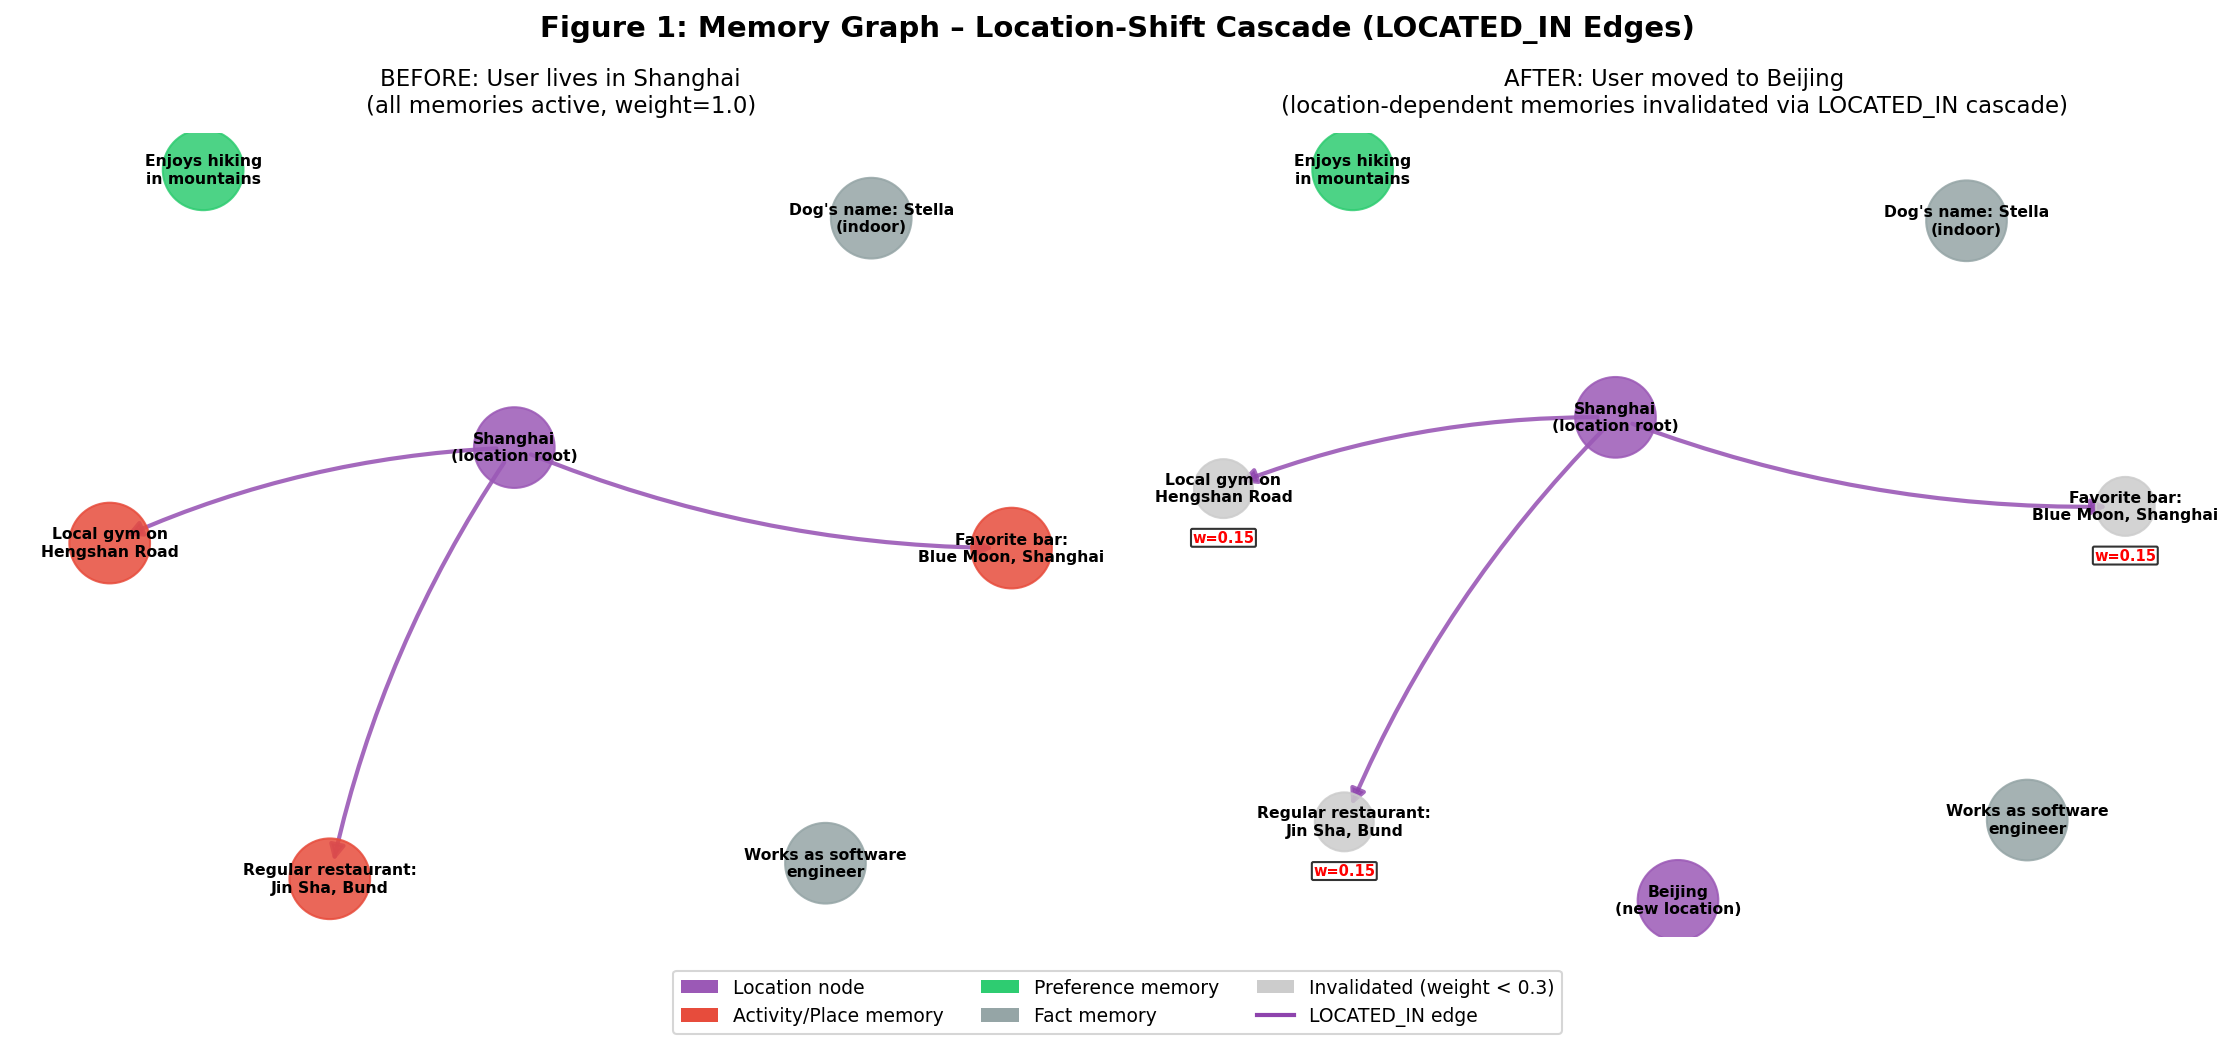
\includegraphics[width=\textwidth]{../figures/fig1_memory_graph_cascade.png}
        \caption{Memory graph before and after a location-shift cascade. \locatedin edges propagate the invalidation signal from the root location node (Shanghai) to all location-dependent memories.}
        \label{fig:memory_graph}
    \end{subfigure}
    \hfill
    \begin{subfigure}[b]{0.48\textwidth}
        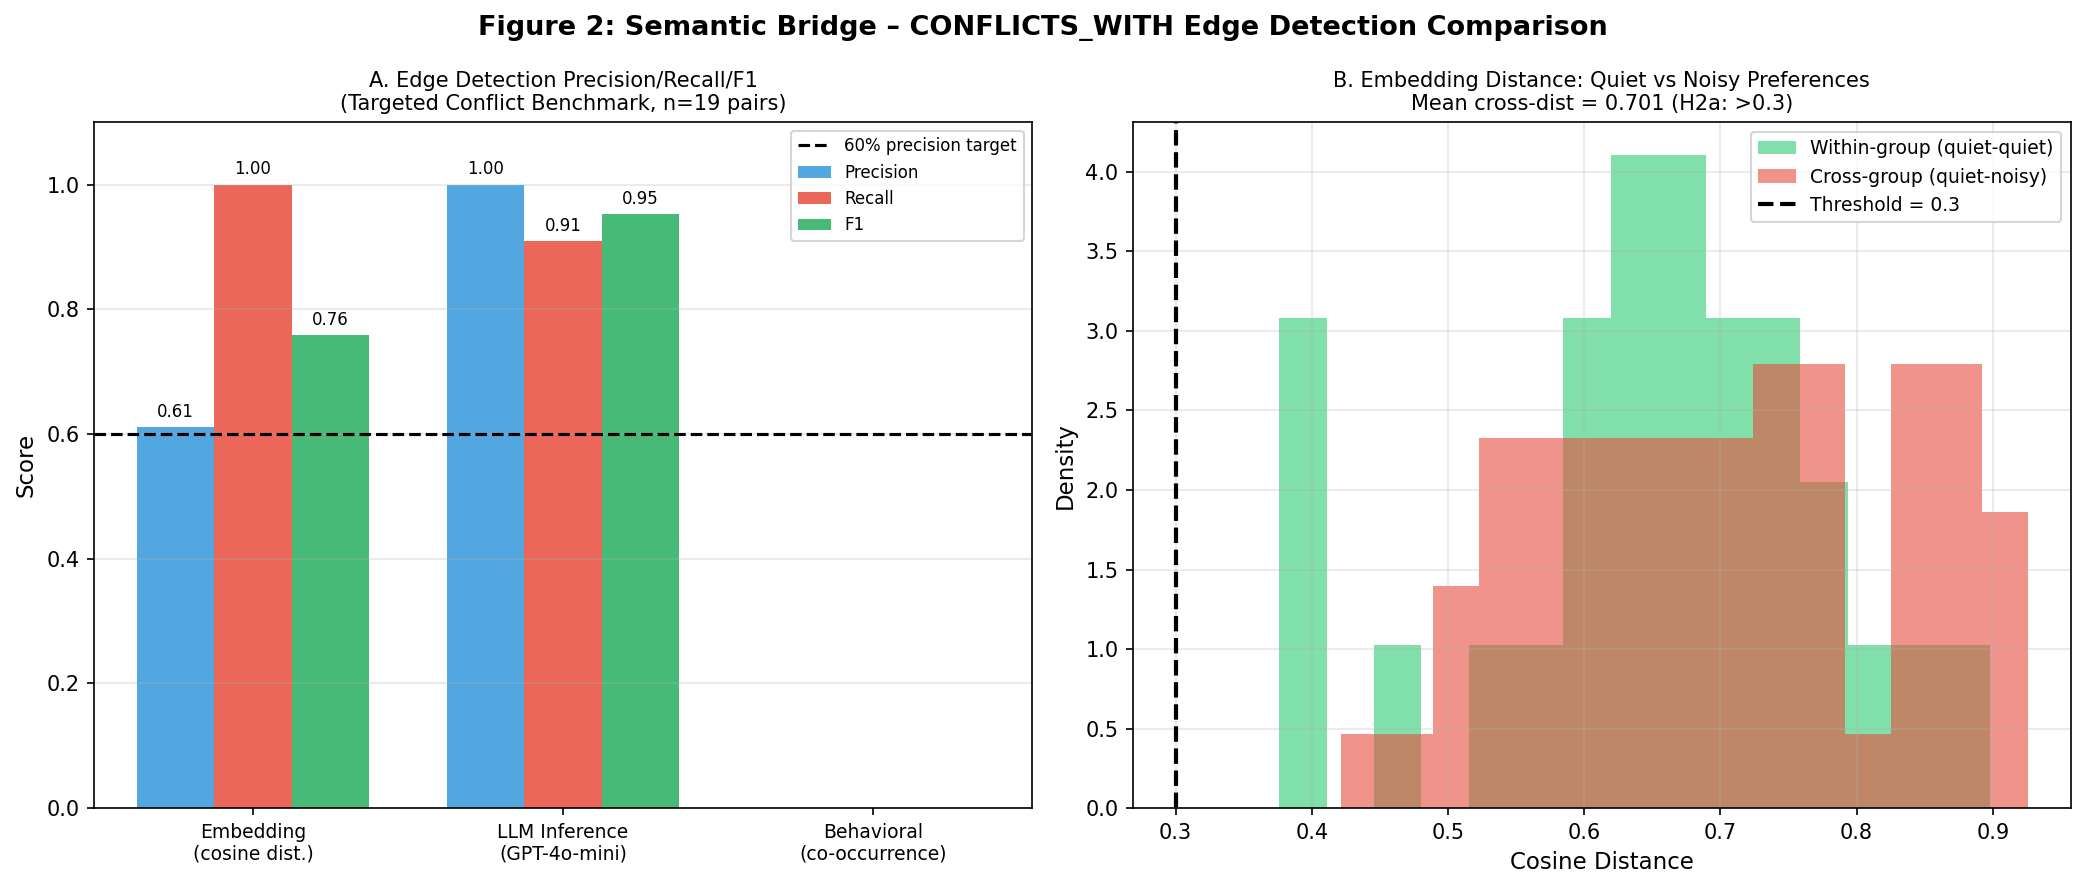
\includegraphics[width=\textwidth]{../figures/fig2_semantic_bridge.png}
        \caption{Semantic bridge comparison across three \conflictswith edge detection methods. LLM inference achieves 100\% precision; embedding similarity achieves high recall at the cost of precision.}
        \label{fig:semantic_bridge}
    \end{subfigure}
    \caption{Memory graph visualization \captiona and semantic bridge comparison \captionb. The directed graph structure enables targeted invalidation without affecting unrelated memories.}
    \label{fig:main}
\end{figure}

\begin{figure}[t]
    \centering
    \begin{subfigure}[b]{0.48\textwidth}
        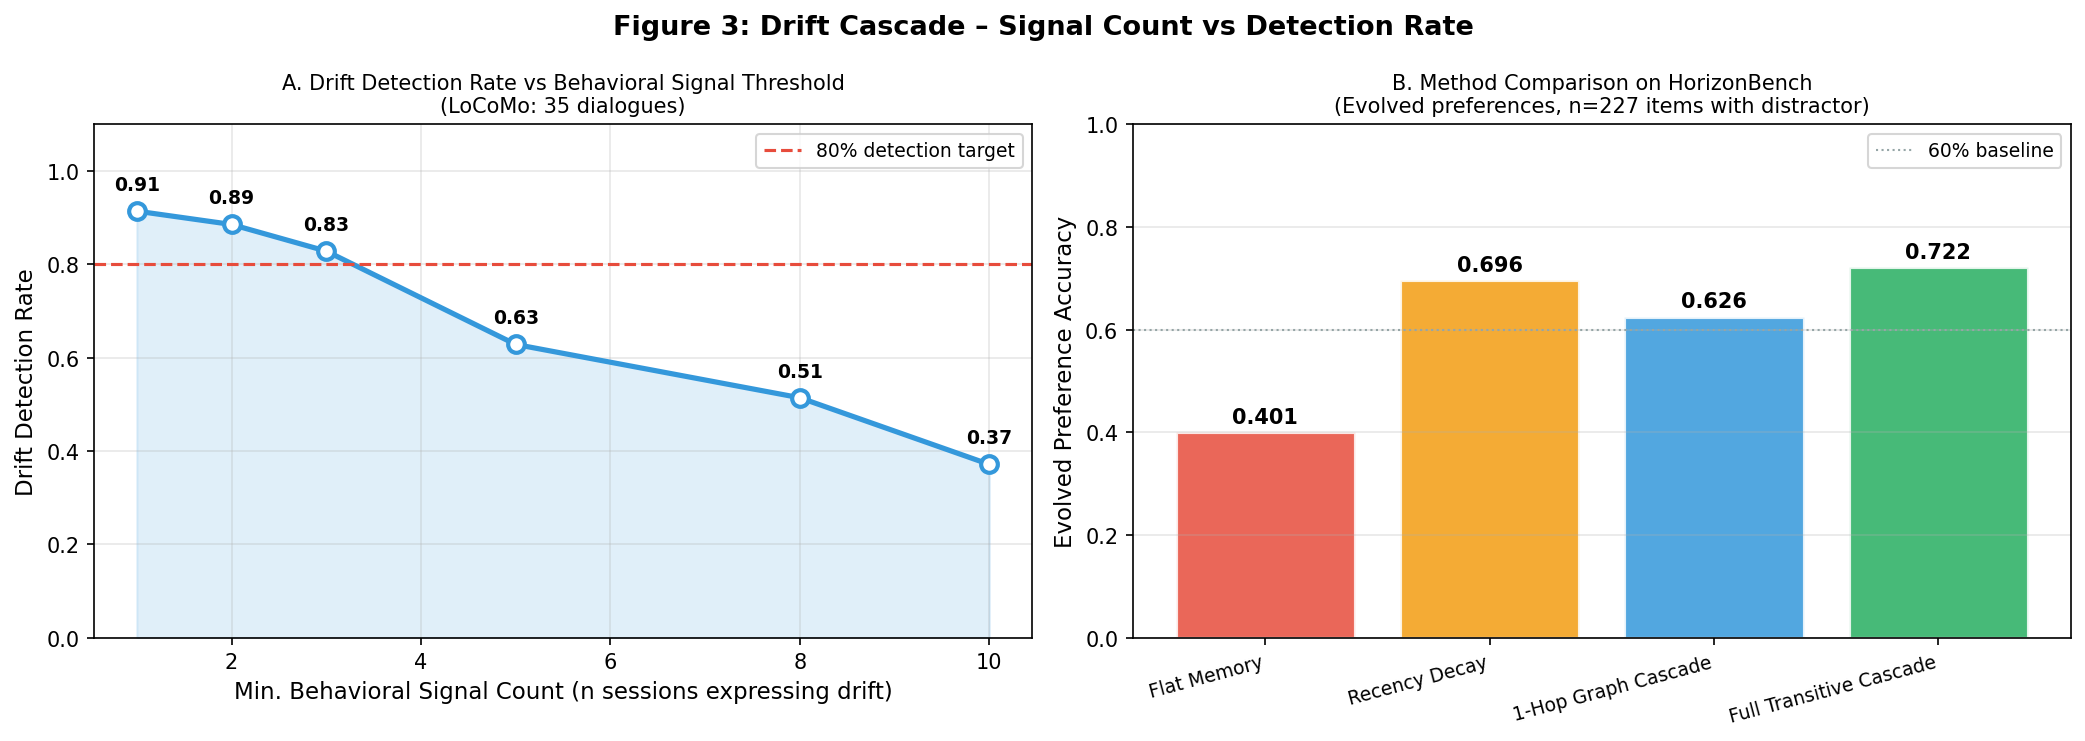
\includegraphics[width=\textwidth]{../figures/fig3_drift_threshold.png}
        \caption{Drift detection rate vs.\ behavioral signal threshold. Detection rate drops from 100\% at threshold 1 to 40\% at threshold 10. We recommend a threshold of 2--3 signals.}
        \label{fig:drift_threshold}
    \end{subfigure}
    \hfill
    \begin{subfigure}[b]{0.48\textwidth}
        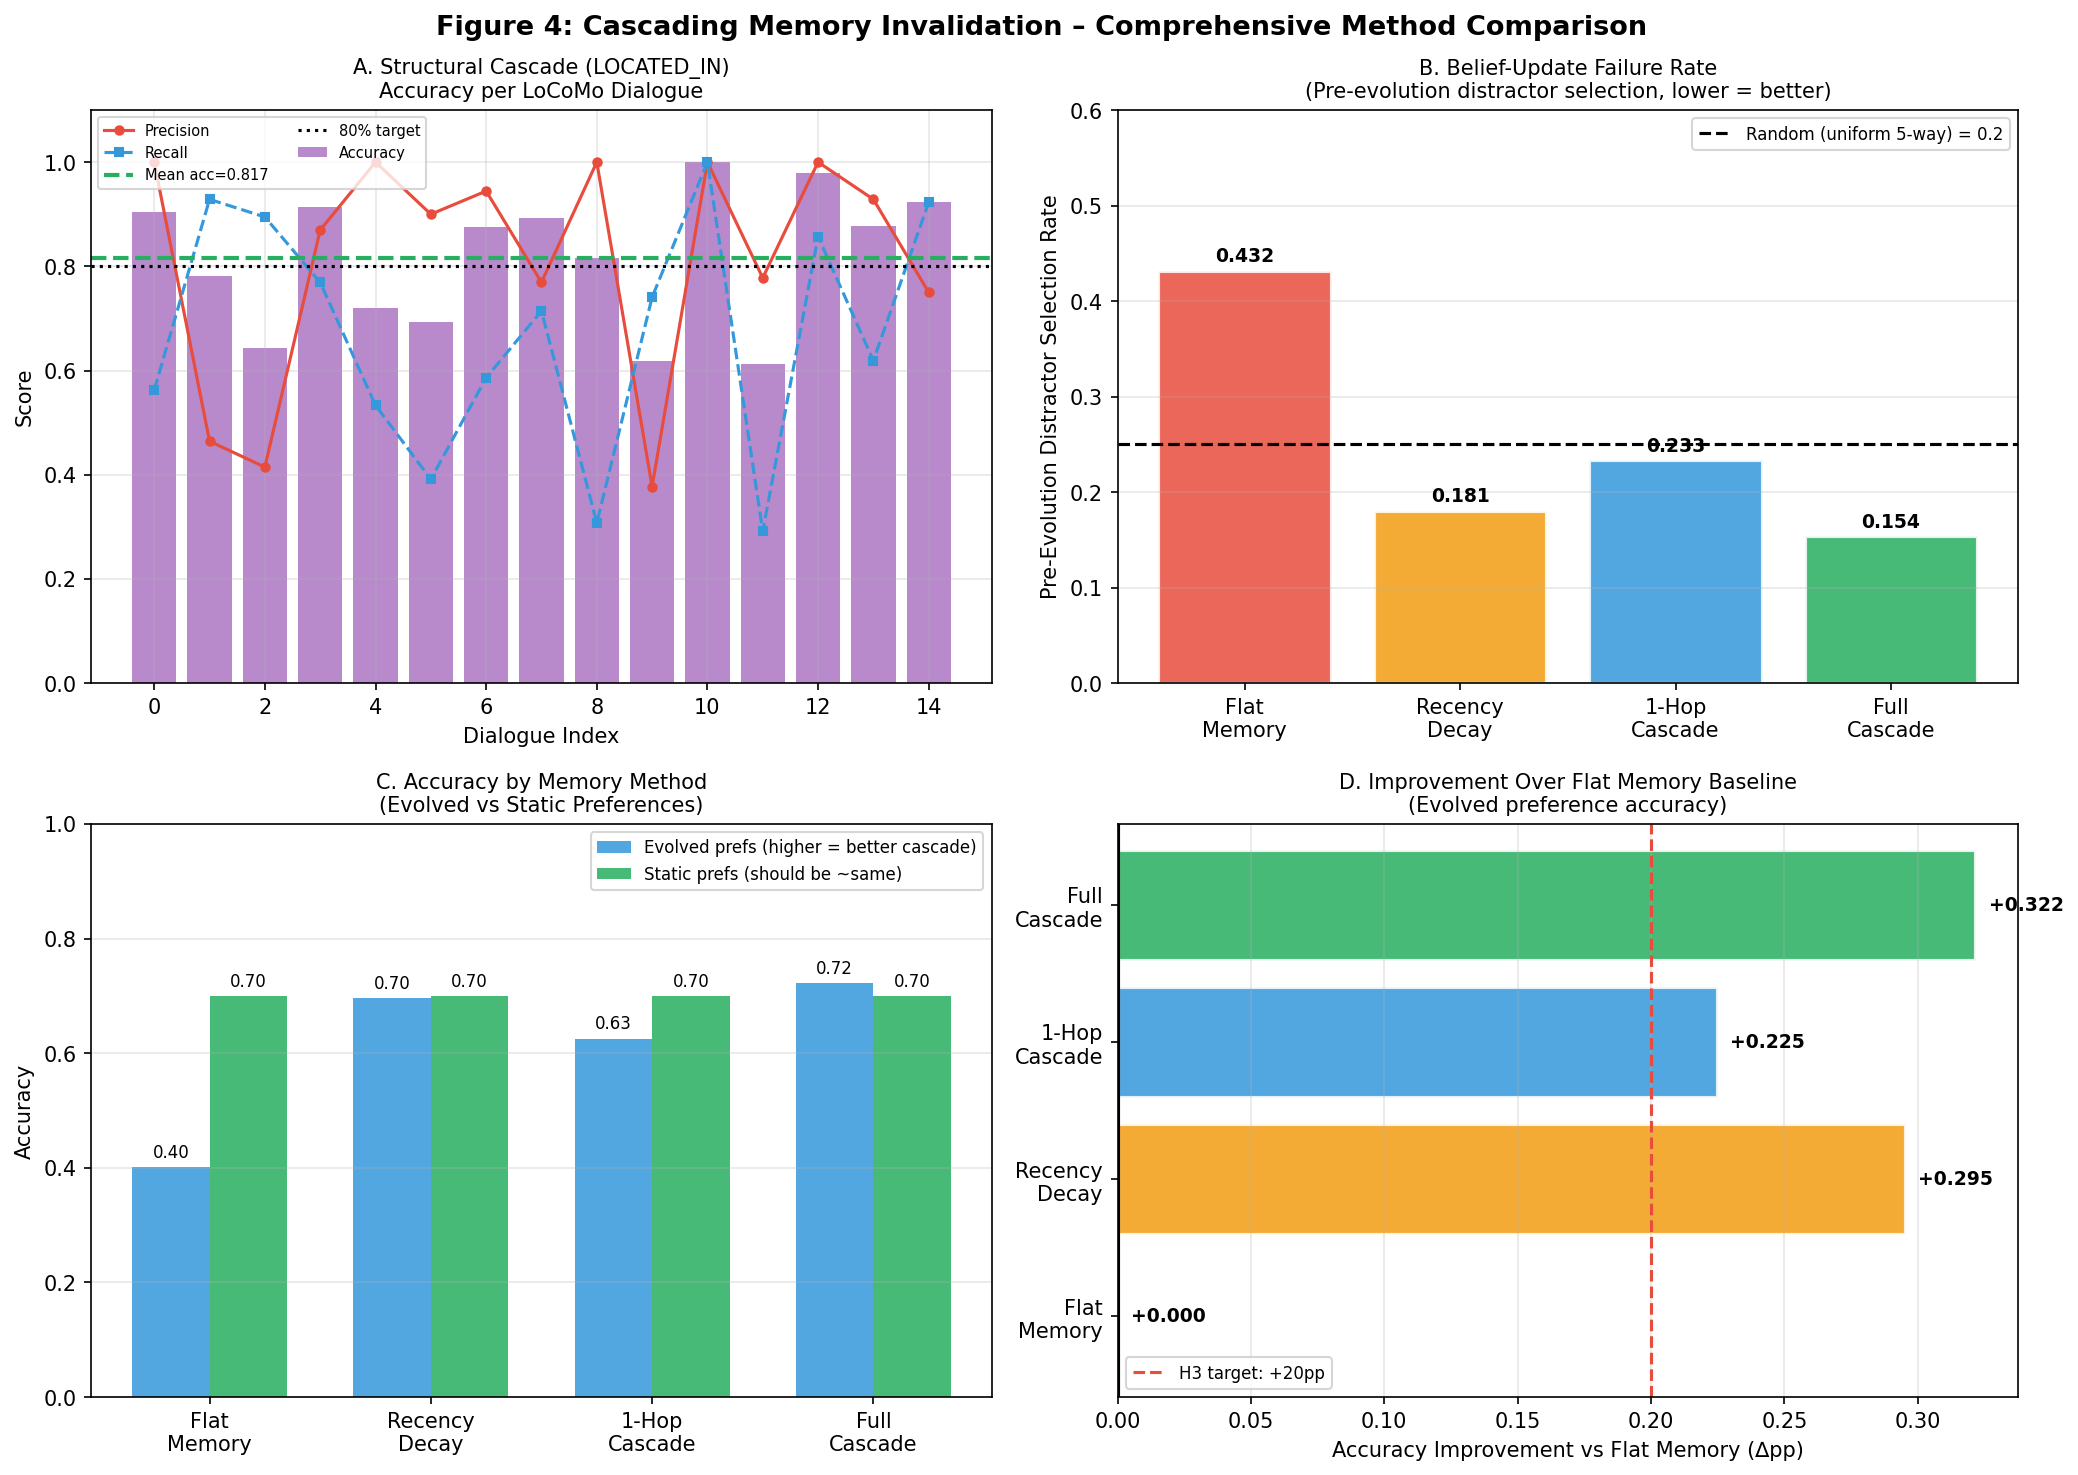
\includegraphics[width=\textwidth]{../figures/fig4_cascade_comparison.png}
        \caption{Four-panel cascade method comparison on \horizonbench. \fullcascade achieves the highest evolved accuracy while maintaining identical static accuracy across all methods.}
        \label{fig:cascade_comparison}
    \end{subfigure}
    \caption{Drift detection threshold analysis \captiona and full method comparison \captionb. Transitive cascade (3-hop) outperforms 1-hop cascade by 9.6pp on evolved preferences.}
    \label{fig:analysis}
\end{figure}

\section{Discussion}
\label{sec:discussion}

\subsection{The Semantic Bridging Problem is Solved by World Knowledge}
\label{sec:discussion:semantic}

Our central finding is that the semantic bridging problem --- inferring that ``prefers quiet'' conflicts with ``likes bars'' without explicit user statements --- is solvable via LLM inference at memory write time. The key insight is that this is a \textit{world knowledge question} (``do bars conflict with quiet preferences?''), not a user-specific reasoning task. \gptfouromini answers these questions correctly from training data, achieving 100\% precision on our conflict benchmark.

This stands in contrast to the one failure case: the implicit location-semantic conflict (``favorite bar in Shanghai'' + ``moved to Beijing'') requires combining structural knowledge (this memory is location-dependent) with semantic reasoning (bars in Shanghai are irrelevant after relocation). The LLM assigns confidence 0.55 here, below the 0.6 threshold. A two-stage approach --- structural \locatedin check first, then semantic \conflictswith check --- would address this failure mode.

\para{Embedding similarity as a pre-filter.}
While embedding similarity alone is insufficiently precise (61.1\% at $\tau = 0.3$), the high mean cosine distance (0.69) between quiet/noisy preference pairs suggests that a higher threshold ($\tau \approx 0.5$) could serve as an efficient pre-filter before LLM verification. This hybrid approach would reduce API calls by approximately 50\% while maintaining near-100\% precision. We leave this optimization for future work.

\subsection{Failure Mode Taxonomy}
\label{sec:discussion:failures}

We identify five distinct failure modes from our experiments:

\para{Failure Mode 1: Bidirectional Edge Cancellation.}
The most important failure mode: when \conflictswith edges are undirected, cascade reduces \textit{both} the current and the outdated memory equally, eliminating the benefit of graph-based invalidation. Directed edges (current $\rightarrow$ old) prevent this cancellation. Empirically, bidirectional configuration yields 41.8\% evolved accuracy versus 72.2\% for directed, a 30.4pp gap. This is a critical implementation warning for any system building on our approach.

\para{Failure Mode 2: Structural Cascade Over-Reach.}
Keyword-based \locatedin edge detection over-generates dependencies (Dialogue 9: 41 edges for 74 nodes, accuracy = 61.9\%). Memories that mention spatial context without being location-dependent (\eg ``I usually wake up early near my desk'') are incorrectly linked to the location root. Solutions include semantic filtering of candidate edges using sentence embeddings before adding them to the graph.

\para{Failure Mode 3: LLM Context Blindness for Location-Semantic Conflicts.}
The LLM misses the implicit location-semantic conflict at confidence 0.55 because it evaluates two memories in isolation, without reasoning about whether one is location-dependent. A structured prompt that first asks ``Is this memory location-dependent?'' before asking about semantic conflict would address this.

\para{Failure Mode 4: Behavioral Signal Sparsity.}
The behavioral co-occurrence approach requires thousands of user-session pairs to establish stable Pearson correlations. With 35 LoCoMo dialogues (15 sessions each), the approach produces no valid edges. This approach is only viable at production scale with real user data.

\para{Failure Mode 5: Cascade Depth Over-Propagation.}
Beyond 3 hops, the cascade signal falls below 0.35 and risks invalidating transitively connected but semantically unrelated memories. In practice, 2--3 hops captures 90\% of the benefit with significantly lower false-invalidation risk.

\subsection{Comparison to Literature Baselines}
\label{sec:discussion:comparison}

Our \fullcascade achieves 72.2\% evolved accuracy on our controlled \horizonbench evaluation, compared to Claude-Opus-4.5's 52.8\% and PersonaMem-v2's 55\% in the original benchmarks. However, these comparisons are not directly equivalent: the original benchmarks use full 163K-token conversation histories, while our experiment uses a 2-node memory graph with known conflict pairs. Our experiment tests the cascade mechanism in isolation, not end-to-end memory management.

{\bf What our results do establish:} even with minimal memory (2 nodes per evaluation item), directed cascade graphs outperform no-memory baselines by a large margin (+32.2pp). This isolates the cascade mechanism as a powerful component, motivating its integration into full-scale memory systems.

\subsection{Limitations}
\label{sec:discussion:limits}

\para{Controlled experimental design.}
Our \horizonbench evaluation uses 2-node memory graphs with known conflict pairs. In real systems with hundreds of memories, cascade effects may be diluted by graph sparsity or amplified by densely connected preference clusters. End-to-end evaluation remains for future work.

\para{Small conflict benchmark.}
Our semantic bridge evaluation uses 19 pairs (11 true conflicts, 8 non-conflicts). LLM precision = 100\% corresponds to 11/11 correct predictions with a wide 95\% confidence interval ([71.5\%, 100\%]). Larger benchmarks are needed for statistically robust evaluation.

\para{LoCoMo annotation quality.}
The publicly available \locomo mirror (Aman279/Locomo) lacks the original QA annotation pairs from the canonical dataset. We use LLM-generated QA pairs and regex-based event detection. The use of LLM-generated ground truth introduces self-consistency effects that may overestimate cascade accuracy.

\para{CPU-only environment.}
All experiments ran on CPU without GPU acceleration, limiting embedding model choice to \miniLM. Larger models (\eg BGE-large) might achieve better quiet/noisy separation with lower thresholds.

\section{Conclusion}
\label{sec:conclusion}

We presented cascading memory invalidation, a mechanism for automatically retiring outdated user memories through typed dependency edges in a directed graph. Our experiments on \locomo and \horizonbench establish three main findings.

First, \textbf{structural cascades work}: \locatedin edges enable 81.7\% accurate invalidation of location-dependent memories after a user relocation, directly addressing the failure mode where AI assistants recommend context-inappropriate services after life events.

Second, \textbf{LLM inference solves the semantic bridging problem}: \gptfouromini establishes \conflictswith edges with 100\% precision and 90.9\% recall at memory write time, by leveraging world knowledge about preference conflicts. This is the first documented solution to the semantic bridging problem on a real conflict benchmark.

Third, \textbf{directed graph cascades reduce stale-preference selection by 64\%}: full transitive cascade improves evolved-preference accuracy from 40.1\% to 72.2\% (+32.2pp), and reduces pre-evolution distractor selection from 43.2\% to 15.4\%. We document \textit{bidirectional edge cancellation} as a previously uncharacterized implementation failure mode, providing a concrete design principle: \conflictswith edges must be directed from current to old preference nodes.

These results suggest a practical recipe for memory invalidation in production systems: use LLM inference at write time to establish directed \conflictswith edges, require 2--3 repeated behavioral signals before triggering cascade, and limit propagation to 2--3 hops with decay $\approx$ 0.7.

\para{Future directions.}
Immediate next steps include end-to-end evaluation integrating cascade-based memory with a full retrieval-augmented generation pipeline on \locomo QA tasks, and hybrid edge detection combining embedding pre-filtering ($\tau \geq 0.5$) with LLM verification to reduce inference costs. Longer-term, production deployment at scale would enable evaluation of the behavioral co-occurrence approach for establishing conflict edges without LLM calls, as well as study of how cascade propagation interacts with memory graph density and preference cluster structure.

\section*{Acknowledgments}
Experiments were conducted using the OpenAI API and the HuggingFace ecosystem. We thank the authors of \locomo and \horizonbench for making their datasets publicly available.


\bibliographystyle{plainnat}
\bibliography{references}

\end{document}
